% !TeX program = xelatex
\documentclass[a4paper,10pt]{article}

% ============================================================================
% កញ្ចប់សម្ភារៈសិក្សាបោះពុម្ព ស-ខ្មៅ (Printable Classroom Materials - Grade 8 2.2 EXP_MUL)
% ត្រូវគ្នា ១០០% នឹង LS_Plan_EXP_MUL.tex, Teaching_Scenario_EXP_MUL.tex និង Teaching_Guideline_EXP_MUL.tex
% ============================================================================
\usepackage[a4paper, left=1.0cm, right=1.0cm, top=0.75cm, bottom=1.05cm, footskip=0.55cm]{geometry}
\usepackage{amsmath, amssymb}
\usepackage{unicode-math}
\usepackage{fontspec}
\usepackage{array, colortbl}
\usepackage[table]{xcolor}
\usepackage{enumitem}
\usepackage{pifont}
\usepackage{fancyhdr}
\usepackage{lastpage}
\usepackage{tikz}
\usepackage[most]{tcolorbox}
\usetikzlibrary{calc, arrows.meta, decorations.markings, positioning, babel}

% LaTeX 2025 compatibility guard
\makeatletter
\let\@expl@@@mark@update@singlecol@structures@@\relax
\makeatother

% ============================================================================
% ការកំណត់ពុម្ពអក្សរផ្លូវការ (Word-Styled Khmer + Cambria Math + Times New Roman)
% ============================================================================
\providecommand{\NGSFindFonts}{%
  \IfFileExists{C:/Windows/Fonts/cambria.ttc}{%
    \def\NGSSysPath{C:/Windows/Fonts/}%
    \def\NGSUserPath{C:/Users/KIT/AppData/Local/Microsoft/Windows/Fonts/}%
  }{%
    \IfFileExists{./fonts/KhmerOSsiemreap.ttf}{\def\NGSSysPath{./fonts/}\def\NGSUserPath{./fonts/}}{%
    \IfFileExists{../fonts/KhmerOSsiemreap.ttf}{\def\NGSSysPath{../fonts/}\def\NGSUserPath{../fonts/}}{%
    \IfFileExists{../../fonts/KhmerOSsiemreap.ttf}{\def\NGSSysPath{../../fonts/}\def\NGSUserPath{../../fonts/}}{%
    \IfFileExists{../../../fonts/KhmerOSsiemreap.ttf}{\def\NGSSysPath{../../../fonts/}\def\NGSUserPath{../../../fonts/}}{%
    \IfFileExists{../../../../fonts/KhmerOSsiemreap.ttf}{\def\NGSSysPath{../../../../fonts/}\def\NGSUserPath{../../../../fonts/}}{%
    \IfFileExists{../../../../../fonts/KhmerOSsiemreap.ttf}{\def\NGSSysPath{../../../../../fonts/}\def\NGSUserPath{../../../../../fonts/}}{%
    \IfFileExists{../../../../../../fonts/KhmerOSsiemreap.ttf}{\def\NGSSysPath{../../../../../../fonts/}\def\NGSUserPath{../../../../../../fonts/}}{%
      \def\NGSSysPath{../../../../../../../fonts/}\def\NGSUserPath{../../../../../../../fonts/}%
    }}}}}}}%
  }%
}
\NGSFindFonts

\setmathfont[
  Path={\NGSSysPath},
  FontIndex=1,
  Scale=1.02
]{cambria.ttc}

\defaultfontfeatures{Ligatures=TeX}

\setmainfont[
  Path={\NGSUserPath},
  Extension=.ttf,
  Script=Khmer,
  BoldFont={KhmerOSsiemreap},
  BoldFeatures={FakeBold=1.8},
  ItalicFont={KhmerOSsiemreap},
  ItalicFeatures={FakeSlant=0.25},
  BoldItalicFont={KhmerOSsiemreap},
  BoldItalicFeatures={FakeBold=1.8, FakeSlant=0.25}
]{KhmerOSsiemreap}

\newfontfamily\muol[
  Path={\NGSUserPath},
  Extension=.ttf,
  Script=Khmer
]{KhmerOSmuollight}

\newfontfamily\TimesEn[
  Path={\NGSSysPath},
  Extension=.ttf,
  BoldFont={timesbd},
  ItalicFont={timesi},
  BoldItalicFont={timesbi}
]{times}

\newfontfamily\CalibriFont[
  Path={\NGSSysPath},
  Extension=.ttf
]{calibri}

\newfontfamily\Tacteing[
  Path={\NGSUserPath}
]{TACTENG.TTF}

\XeTeXlinebreaklocale "km"
\XeTeXlinebreakskip = 0pt plus 1pt minus 0.1pt

% ============================================================================
% ក្ដារពណ៌ ស-ខ្មៅ សុទ្ធសម្រាប់ការបោះពុម្ព (Strict Monochrome Print Palette)
% ============================================================================
\definecolor{panelgray}{gray}{0.92} % ~gray!8
\definecolor{headgray}{gray}{0.85}  % ~gray!15
\definecolor{midgray}{gray}{0.75}   % ~gray!25
\definecolor{darkline}{gray}{0.35}  % ~gray!65

\pagestyle{fancy}
\fancyhf{}
\renewcommand{\headrulewidth}{0pt}
\fancyfoot[L]{\fontsize{6.9pt}{9pt}\selectfont អនុវិទ្យាល័យព្រះក្រសាំង \en{---} គណិតវិទ្យា ថ្នាក់ទី៨ \en{|} មេរៀនទី២ (២\en{.}២) វិធីគុណស្វ័យគុណមាននិទស្សន្តរ៉ឺឡាទីប (ស-ខ្មៅ) \en{|} ថ្ងៃចន្ទ ៧កើត កត្តិក ២៥៧០ \en{|} ថ្ងៃទី១៦ ខែវិច្ឆិកា ឆ្នាំ២០២៦}
\fancyfoot[R]{\fontsize{7.5pt}{9pt}\selectfont ទំព័រ \en{\thepage\ / \pageref{LastPage}}}

\setlength{\parindent}{0pt}
\setlength{\parskip}{0pt}
\setlength{\tabcolsep}{4pt}

% ============================================================================
% ម៉ាក្រូជំនួយ (Helper Macros)
% ============================================================================
\newcommand{\en}[1]{{\TimesEn #1}}
\newcommand{\enbf}[1]{{\TimesEn\bfseries #1}}
\newcommand{\unit}[1]{\,\text{\en{#1}}}
\newcommand{\cnum}[1]{\mbox{\normalfont\fontsize{10pt}{12pt}\selectfont\ding{\numexpr181+#1\relax}}}
\newcommand{\blankcnum}{\tikz[baseline=-0.35ex]\draw[black, line width=0.8pt] (0,0) circle (0.175cm);}
\newcommand{\expbox}{\tikz[baseline=-0.1ex]\draw[black, line width=0.65pt, fill=white] (0,0) rectangle (0.34cm,0.22cm);}
\newcommand{\scissors}{\ding{34}}
\newcommand{\chkbox}{\tikz[baseline=-0.15ex]\draw[black, line width=0.85pt] (0,0) rectangle (0.24cm,0.24cm);}
\newcommand{\circbox}[1]{\tikz[baseline=(c.base)]\node[draw=black, rounded corners=4pt, line width=0.8pt, inner sep=1.4pt] (c) {\ensuremath{#1}};}
\newcommand{\khmflourish}{{\Tacteing\fontsize{32pt}{13pt}\selectfont\raisebox{-4pt}{3}}}

\newcommand{\pagebanner}[2]{%
  \begin{tcolorbox}[
    enhanced, sharp corners, colback=headgray, colframe=black,
    boxrule=1.1pt, boxsep=1pt, top=3pt, bottom=3pt, left=6pt, right=6pt,
    after skip=4pt
  ]
    {\muol\fontsize{9.0pt}{13.4pt}\selectfont #1}\hfill{\fontsize{8.0pt}{11.5pt}\selectfont\textbf{#2}}
  \end{tcolorbox}%
}

\newcolumntype{L}[1]{>{\raggedright\arraybackslash}p{#1}}
\newcolumntype{C}[1]{>{\centering\arraybackslash}p{#1}}

\begin{document}
\fontsize{9.0pt}{13.2pt}\selectfont

% ============================================================================
% ទំព័រទី ១៖ សម្ភារៈ E2 ខ្នាតពិត 1:1 (បន្ទះកត្តា 2^3, 2^4 + បន្សាបគូសូន្យ 10^-3 x 10^4 + Dual POE 2A-2B)
% ============================================================================
\pagebanner{សម្ភារៈទី ១៖ បន្ទះកាត់ \enbf{E2} ខ្នាតពិត \enbf{1:1} «កត្តាគុណ និងគូសូន្យ» \enbf{\&} ពិសោធន៍ \enbf{POE 2A--2B}}{ទំព័រ ១/៦ \en{-- E2 Explore}}

% --- ប្រអប់ព្រមានខ្នាតពិត & បន្ទះផ្ទៀង 5.00 cm (x=1cm, y=1cm) ---
\noindent
\begin{minipage}[c]{11.9cm}
  \begin{tcolorbox}[
    enhanced, sharp corners, colback=panelgray, colframe=black,
    boxrule=1.0pt, boxsep=1pt, top=3pt, bottom=3pt, left=6pt, right=6pt
  ]
    \fontsize{8.0pt}{11.2pt}\selectfont
    \textbf{ការណែនាំសំខាន់មុនបោះពុម្ព (\en{Print at 100\% / Actual Size})៖} ពេលបោះពុម្ព សូមជ្រើស \textbf{\en{Scale: Actual Size 100\%}} \en{--} \textbf{កុំជ្រើស \en{Fit to Page}} ដើម្បីឱ្យបន្ទះកត្តា $2^3$ ($3.00\unit{cm}$), $2^4$ ($4.00\unit{cm}$), បន្ទាត់ $0\text{--}8\unit{cm}$ និងផ្ទាំងបន្សាបគូសូន្យត្រូវខ្នាតពិត \en{1:1}។\\[1.5pt]
    \textbf{បេសកកម្មឃ្លាំងវីដេអូ \en{Server (E1)}៖} កាត់បន្ទះ \scissors{} តភ្ជាប់គុណ $2^3 \times 2^4$ លើបន្ទាត់ $0\text{--}8\unit{cm}$ និងគូសឆ្នូត \en{/} បន្សាបគូសូន្យសម្រាប់ទិន្នន័យ $10^{-3} \times 10^4\unit{MB}$។
  \end{tcolorbox}
\end{minipage}%
\hfill
\begin{minipage}[c]{6.8cm}
  \begin{tcolorbox}[
    enhanced, sharp corners, colback=white, colframe=black,
    boxrule=1.0pt, boxsep=1pt, top=2.5pt, bottom=2.5pt, left=4pt, right=4pt
  ]
    \centering
    {\fontsize{8.0pt}{10.2pt}\selectfont\textbf{បន្ទះផ្ទៀងខ្នាតពិត \en{5.00 cm} (\en{Actual Size 100\%})}}\\[2pt]
    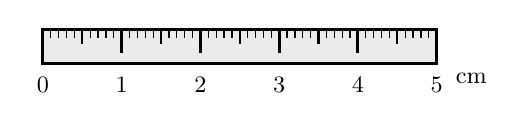
\begin{tikzpicture}[x=1cm, y=1cm, every node/.style={font=\fontsize{8.5pt}{10.5pt}\selectfont, text=black}]
      \draw[black, line width=1.1pt, fill=panelgray] (0,0) rectangle (5.0, 0.44);
      \foreach \m in {0,...,50}{
        \pgfmathsetmacro{\xval}{\m*0.1}
        \draw[black, line width=0.45pt] (\xval, 0.44) -- (\xval, 0.33);
      }
      \foreach \h in {0,0.5,...,5.0}{
        \draw[black, line width=0.8pt] (\h, 0.44) -- (\h, 0.25);
      }
      \foreach \c in {0,1,2,3,4,5}{
        \draw[black, line width=1.1pt] (\c, 0.44) -- (\c, 0.14);
        \node[below=1pt] at (\c, 0.0) {\en{\c}};
      }
      \node[right=2pt] at (5.05, -0.18) {\en{cm}};
    \end{tikzpicture}
  \end{tcolorbox}
\end{minipage}

\vspace{6pt}

% --- ផ្នែកទី ១៖ សកម្មភាព 1 — បន្ទះកត្តា 2^3, 2^4 (1:1) & ផ្ទាំងបន្សាបគូសូន្យ 10^-3 x 10^4 (1:1) ---
\textbf{១. សកម្មភាព \en{1} (\en{6 min}) ៖ បន្ទះកត្តាគុណតភ្ជាប់ ($2^3\times 2^4$) និងផ្ទាំងបន្សាបគូសូន្យ ($10^{-3}\times 10^4$) ខ្នាតពិត \en{1:1} (\en{x=1cm, y=1cm})}

\vspace{4pt}
\noindent
\begin{minipage}[t]{9.25cm}
  \vspace{0pt}
  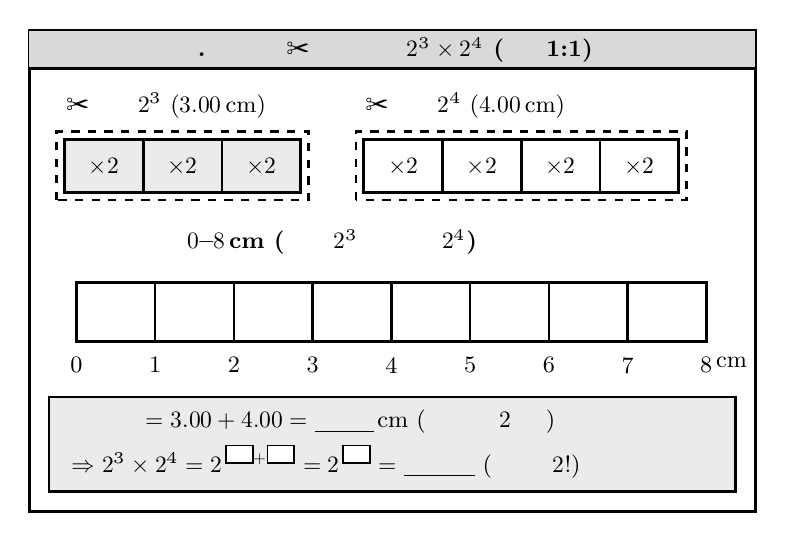
\begin{tikzpicture}[x=1cm, y=1cm, every node/.style={font=\fontsize{8.5pt}{10.5pt}\selectfont, text=black}]
    \draw[black, line width=1.05pt] (0, 0) rectangle (9.22, 6.10);
    \fill[headgray] (0, 5.62) rectangle (9.22, 6.10);
    \draw[black, line width=0.85pt] (0, 5.62) -- (9.22, 5.62);
    \node at (4.61, 5.86) {\textbf{ក. កាត់បន្ទះ \scissors{} តភ្ជាប់កត្តា $2^3 \times 2^4$ (ខ្នាត \en{1:1})}};

    % Strip 2^3 = 3.00 cm (3 boxes x 1.00 cm)
    \node[anchor=west] at (0.35, 5.15) {\scissors\ បន្ទះ $2^3$ ($3.00\unit{cm}$)};
    \draw[black, dashed, line width=0.95pt] (0.35, 3.95) rectangle (3.55, 4.82);
    \draw[black, line width=1.15pt, fill=panelgray] (0.45, 4.05) rectangle (3.45, 4.72);
    \draw[black, line width=1.0pt] (1.45, 4.05) -- (1.45, 4.72);
    \draw[black, line width=1.0pt] (2.45, 4.05) -- (2.45, 4.72);
    \node at (0.95, 4.385) {$\times 2$};
    \node at (1.95, 4.385) {$\times 2$};
    \node at (2.95, 4.385) {$\times 2$};

    % Strip 2^4 = 4.00 cm (4 boxes x 1.00 cm)
    \node[anchor=west] at (4.15, 5.15) {\scissors\ បន្ទះ $2^4$ ($4.00\unit{cm}$)};
    \draw[black, dashed, line width=0.95pt] (4.15, 3.95) rectangle (8.35, 4.82);
    \draw[black, line width=1.15pt, fill=white] (4.25, 4.05) rectangle (8.25, 4.72);
    \draw[black, line width=1.0pt] (5.25, 4.05) -- (5.25, 4.72);
    \draw[black, line width=1.0pt] (6.25, 4.05) -- (6.25, 4.72);
    \draw[black, line width=1.0pt] (7.25, 4.05) -- (7.25, 4.72);
    \node at (4.75, 4.385) {$\times 2$};
    \node at (5.75, 4.385) {$\times 2$};
    \node at (6.75, 4.385) {$\times 2$};
    \node at (7.75, 4.385) {$\times 2$};

    % 0-8 cm Concatenation Track (exact 8.00 cm from x=0.60 to x=8.60)
    \node[anchor=west] at (0.35, 3.42) {\textbf{ផ្លូវតភ្ជាប់កត្តា $0\text{--}8\unit{cm}$ (តម្រៀប $2^3$ រួចតភ្ជាប់ $2^4$)៖}};
    \draw[black, line width=1.15pt] (0.60, 2.15) rectangle (8.60, 2.90);
    \foreach \k in {0,1,...,8}{
      \draw[black, line width=0.95pt] ({0.60+\k}, 2.15) -- ({0.60+\k}, 2.90);
      \node[below=2pt] at ({0.60+\k}, 2.15) {\en{\k}};
    }
    \node[below=2pt] at (8.92, 2.15) {\en{cm}};

    % Bottom observation prompt
    \draw[black, line width=0.8pt, fill=panelgray] (0.25, 0.25) rectangle (8.97, 1.45);
    \node[anchor=west, align=left] at (0.42, 0.85)
      {ប្រវែងសរុប $= 3.00 + 4.00 = \underline{\hspace{0.75cm}}\unit{cm}$ (ចំនួនកត្តា $2$ សរុប)\\[3pt]
       $\Rightarrow 2^3 \times 2^4 = 2^{\,\expbox + \expbox} = 2^{\,\expbox} = \underline{\hspace{0.9cm}}$ (រក្សាគោល $2$!)};
  \end{tikzpicture}
\end{minipage}%
\hfill
\begin{minipage}[t]{9.25cm}
  \vspace{0pt}
  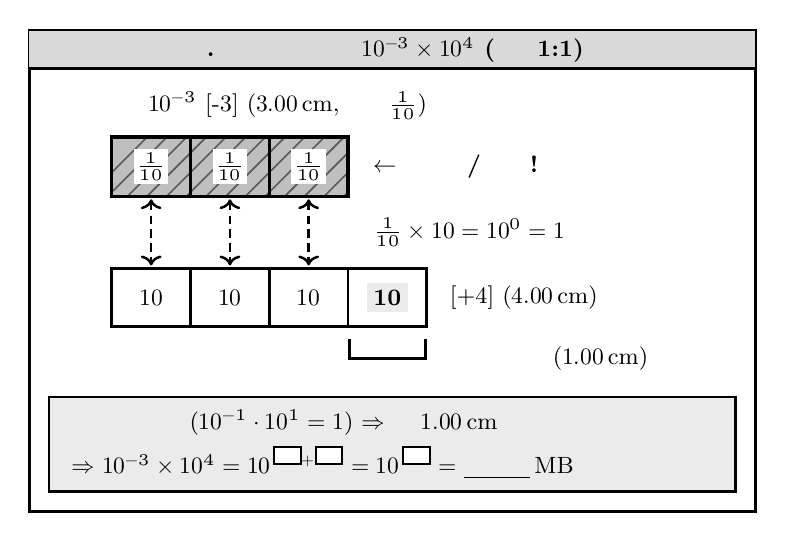
\begin{tikzpicture}[x=1cm, y=1cm, every node/.style={font=\fontsize{8.5pt}{10.5pt}\selectfont, text=black}]
    \draw[black, line width=1.05pt] (0, 0) rectangle (9.22, 6.10);
    \fill[headgray] (0, 5.62) rectangle (9.22, 6.10);
    \draw[black, line width=0.85pt] (0, 5.62) -- (9.22, 5.62);
    \node at (4.61, 5.86) {\textbf{ខ. ផ្ទាំងបន្សាបគូសូន្យ $10^{-3} \times 10^4$ (ខ្នាត \en{1:1})}};

    % 3.00 cm hatched strip for 10^-3 (3 cells of 1/10 = 10^-1)
    \node[anchor=west] at (0.35, 5.15) {\textbf{កាត់តភ្ជាប់ $10^{-3}$} \en{[-3]} ($3.00\unit{cm}$, កត្តា $\frac{1}{10}$)};
    \draw[black, line width=1.15pt, fill=midgray] (1.05, 4.00) rectangle (4.05, 4.75);
    \begin{scope}
      \clip (1.05, 4.00) rectangle (4.05, 4.75);
      \foreach \hx in {0.75, 1.00, ..., 4.45}{
        \draw[darkline, line width=0.6pt] (\hx, 4.00) -- (\hx+0.75, 4.75);
      }
    \end{scope}
    \draw[black, line width=1.15pt] (1.05, 4.00) rectangle (4.05, 4.75);
    \draw[black, line width=1.0pt] (2.05, 4.00) -- (2.05, 4.75);
    \draw[black, line width=1.0pt] (3.05, 4.00) -- (3.05, 4.75);
    \node[fill=white, inner sep=1pt] at (1.55, 4.375) {$\frac{1}{10}$};
    \node[fill=white, inner sep=1pt] at (2.55, 4.375) {$\frac{1}{10}$};
    \node[fill=white, inner sep=1pt] at (3.55, 4.375) {$\frac{1}{10}$};
    \node[anchor=west] at (4.25, 4.375) {$\leftarrow$ \textbf{គូសឆ្នូត \en{/} កាត់គូ!}};

    % 1-to-1 vertical pairing arrows (3 pairs)
    \foreach \px in {1.55, 2.55, 3.55}{
      \draw[black, densely dashed, line width=0.9pt, <->] (\px, 3.96) -- (\px, 3.12);
    }
    \node[anchor=west] at (4.25, 3.54) {$\frac{1}{10} \times 10 = 10^0 = 1$};

    % 4.00 cm solid white strip for 10^4 (4 cells of 10)
    \draw[black, line width=1.15pt, fill=white] (1.05, 2.34) rectangle (5.05, 3.08);
    \draw[black, line width=1.0pt] (2.05, 2.34) -- (2.05, 3.08);
    \draw[black, line width=1.0pt] (3.05, 2.34) -- (3.05, 3.08);
    \draw[black, line width=1.0pt] (4.05, 2.34) -- (4.05, 3.08);
    \node at (1.55, 2.71) {$10$};
    \node at (2.55, 2.71) {$10$};
    \node at (3.55, 2.71) {$10$};
    \node[fill=panelgray, inner sep=2.5pt] at (4.55, 2.71) {\textbf{10}};
    \node[anchor=west] at (5.22, 2.71) {\en{[+4]} ($4.00\unit{cm}$)};

    % Bracket pointing to remaining 1.00 cm cell
    \draw[black, line width=1.0pt] (4.07, 2.18) -- (4.07, 1.94) -- (5.03, 1.94) -- (5.03, 2.18);
    \node[anchor=west] at (5.20, 1.94) {នៅសល់ \textbf{១ ប្រអប់} ($1.00\unit{cm}$)};

    % Bottom observation prompt
    \draw[black, line width=0.8pt, fill=panelgray] (0.25, 0.25) rectangle (8.97, 1.45);
    \node[anchor=west, align=left] at (0.42, 0.85)
      {បន្សាប \textbf{៣ គូសូន្យ} ($10^{-1}\cdot 10^1=1$) $\Rightarrow$ សល់ $1.00\unit{cm}$\\[3pt]
       $\Rightarrow 10^{-3}\times 10^4 = 10^{\,\expbox + \expbox} = 10^{\,\expbox} = \underline{\hspace{0.85cm}}\unit{MB}$};
  \end{tikzpicture}
\end{minipage}

\vspace{7pt}

% --- ផ្នែកទី ២៖ សកម្មភាព 2 (Dual POE 2A & 2B ជាមួយរូបប្លុក/ក្រឡាចត្រង្គបង្វិល ~25 ដឺក្រេ) ---
\textbf{២. សកម្មភាព \en{2} (\en{POE 2A \& 2B -- 5 min}) ៖ អន្ទាក់គុណគោល និងអន្ទាក់គុណនិទស្សន្ត / ភ្លេច \en{1} (\en{x=1cm, y=1cm})}

\vspace{4pt}
\noindent
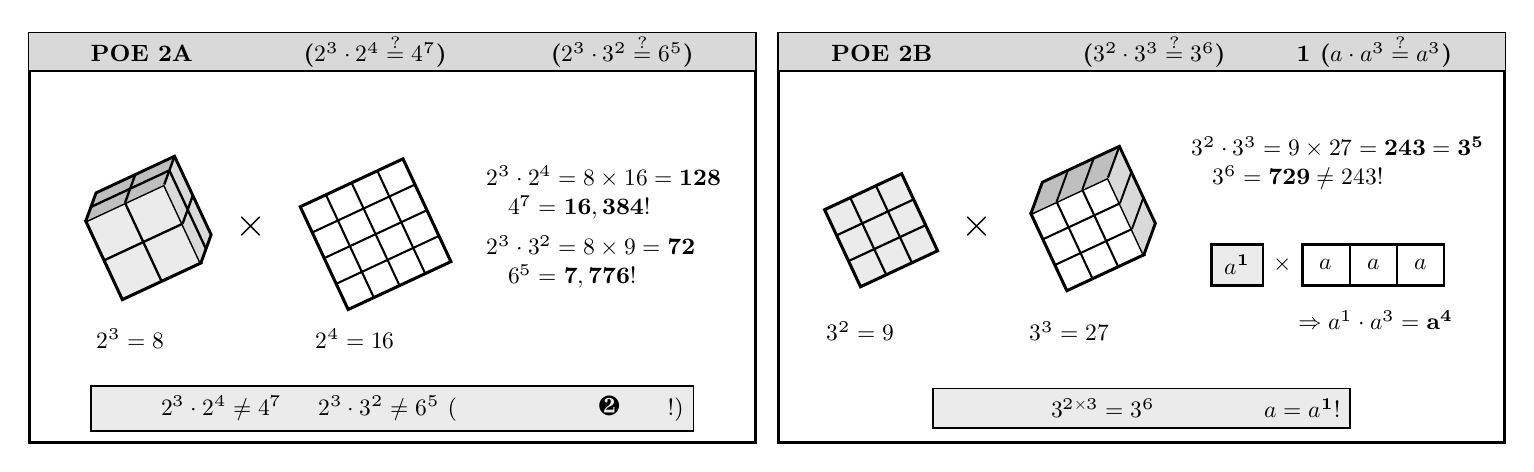
\begin{tikzpicture}[x=1cm, y=1cm, every node/.style={font=\fontsize{8.5pt}{10.5pt}\selectfont, text=black}]
  % === Panel POE 2A: Base Multiplication & Unlike-Base Traps with ~25 deg rotated B&W blocks ===
  \begin{scope}[shift={(0,0)}]
    \draw[black, line width=1.05pt] (0, 0) rectangle (9.22, 5.20);
    \fill[headgray] (0, 4.72) rectangle (9.22, 5.20);
    \draw[black, line width=0.85pt] (0, 4.72) -- (9.22, 4.72);
    \node at (4.61, 4.96) {\textbf{\en{POE 2A}៖ អន្ទាក់គុណគោល ($2^3\cdot 2^4 \stackrel{?}{=} 4^7$) និងគោលខុសគ្នា ($2^3\cdot 3^2 \stackrel{?}{=} 6^5$)}};

    % Rotated ~25 deg 2x2x2 cube (2^3 = 8)
    \begin{scope}[shift={(1.45, 2.55)}, rotate=25]
      \fill[panelgray] (-0.55,-0.55) rectangle (0.55,0.55);
      \draw[black, line width=1.1pt] (-0.55,-0.55) rectangle (0.55,0.55);
      \draw[black, line width=0.85pt] (0,-0.55)--(0,0.55) (-0.55,0)--(0.55,0);
      \fill[midgray] (-0.55,0.55)--(0.55,0.55)--(0.82,0.82)--(-0.28,0.82)--cycle;
      \fill[headgray] (0.55,-0.55)--(0.82,-0.28)--(0.82,0.82)--(0.55,0.55)--cycle;
      \draw[black, line width=1.05pt] (-0.55,0.55)--(-0.28,0.82)--(0.82,0.82)--(0.82,-0.28)--(0.55,-0.55);
      \draw[black, line width=0.85pt] (0.55,0.55)--(0.82,0.82) (0,0.55)--(0.27,0.82) (-0.415,0.685)--(0.685,0.685);
      \draw[black, line width=0.85pt] (0.55,0)--(0.82,0.27) (0.685,-0.415)--(0.685,0.685);
    \end{scope}
    \node at (1.55, 1.32) {$2^3 = 8$ ប្លុក};

    \node at (2.82, 2.75) {\Large $\times$};

    % Rotated ~25 deg 4x4 grid (2^4 = 16)
    \begin{scope}[shift={(4.40, 2.65)}, rotate=25]
      \fill[white] (-0.72,-0.72) rectangle (0.72,0.72);
      \draw[black, line width=1.1pt] (-0.72,-0.72) rectangle (0.72,0.72);
      \foreach \g in {-0.36, 0, 0.36}{
        \draw[black, line width=0.75pt] (\g, -0.72)--(\g, 0.72) (-0.72, \g)--(0.72, \g);
      }
    \end{scope}
    \node at (4.40, 1.32) {$2^4 = 16$ ក្រឡា};

    \node[align=left] at (7.30, 2.80)
      {\textbf{ផ្ទៀងខ្នាតតម្លៃពិត៖}\\
       $2^3 \cdot 2^4 = 8 \times 16 = \mathbf{128}$\\
       តែ $4^7 = \mathbf{16,384}$!\\[4pt]
       $2^3 \cdot 3^2 = 8 \times 9 = \mathbf{72}$\\
       តែ $6^5 = \mathbf{7,776}$!};

    \node[fill=panelgray, draw=black, line width=0.7pt, inner sep=3.5pt] at (4.61, 0.44) {បញ្ជាក់៖ $2^3\cdot 2^4 \neq 4^7$ និង $2^3\cdot 3^2 \neq 6^5$ (គោលខុសគ្នា ប្រើវិធាន \cnum{2} មិនបាន!)};
  \end{scope}

  % === Panel POE 2B: Exponent Multiplication & Hidden Exponent 1 with ~25 deg rotated B&W grids ===
  \begin{scope}[shift={(9.52,0)}]
    \draw[black, line width=1.05pt] (0, 0) rectangle (9.22, 5.20);
    \fill[headgray] (0, 4.72) rectangle (9.22, 5.20);
    \draw[black, line width=0.85pt] (0, 4.72) -- (9.22, 4.72);
    \node at (4.61, 4.96) {\textbf{\en{POE 2B}៖ អន្ទាក់គុណនិទស្សន្ត ($3^2\cdot 3^3 \stackrel{?}{=} 3^6$) និងភ្លេច \en{1} ($a\cdot a^3 \stackrel{?}{=} a^3$)}};

    % Rotated ~25 deg 3x3 grid (3^2 = 9)
    \begin{scope}[shift={(1.30, 2.70)}, rotate=25]
      \fill[panelgray] (-0.54,-0.54) rectangle (0.54,0.54);
      \draw[black, line width=1.1pt] (-0.54,-0.54) rectangle (0.54,0.54);
      \draw[black, line width=0.8pt] (-0.18,-0.54)--(-0.18,0.54) (0.18,-0.54)--(0.18,0.54);
      \draw[black, line width=0.8pt] (-0.54,-0.18)--(0.54,-0.18) (-0.54,0.18)--(0.54,0.18);
    \end{scope}
    \node at (1.30, 1.42) {$3^2 = 9$ ក្រឡា};

    \node at (2.52, 2.75) {\Large $\times$};

    % Rotated ~25 deg 3x3x3 cube (3^3 = 27)
    \begin{scope}[shift={(3.92, 2.65)}, rotate=25]
      \fill[white] (-0.54,-0.54) rectangle (0.54,0.54);
      \draw[black, line width=1.1pt] (-0.54,-0.54) rectangle (0.54,0.54);
      \draw[black, line width=0.75pt] (-0.18,-0.54)--(-0.18,0.54) (0.18,-0.54)--(0.18,0.54);
      \draw[black, line width=0.75pt] (-0.54,-0.18)--(0.54,-0.18) (-0.54,0.18)--(0.54,0.18);
      \fill[midgray] (-0.54,0.54)--(0.54,0.54)--(0.84,0.84)--(-0.24,0.84)--cycle;
      \fill[headgray] (0.54,-0.54)--(0.84,-0.24)--(0.84,0.84)--(0.54,0.54)--cycle;
      \draw[black, line width=1.05pt] (-0.54,0.54)--(-0.24,0.84)--(0.84,0.84)--(0.84,-0.24)--(0.54,-0.54);
      \draw[black, line width=0.75pt] (0.54,0.54)--(0.84,0.84);
      \draw[black, line width=0.7pt] (-0.18,0.54)--(0.12,0.84) (0.18,0.54)--(0.48,0.84);
      \draw[black, line width=0.7pt] (0.54,-0.18)--(0.84,0.12) (0.54,0.18)--(0.84,0.48);
    \end{scope}
    \node at (3.95, 1.42) {$3^3 = 27$ ប្លុក};

    % Right side: 3^5 vs 3^6 and hidden exponent 1 block diagram (a^1 * a^3 = a^4)
    \node[align=left] at (7.10, 3.55)
      {$3^2\cdot 3^3 = 9\times 27 = \mathbf{243} = \mathbf{3^5}$\\
       តែ $3^6 = \mathbf{729} \neq 243$!};
    % Hidden exponent 1 box visual
    \draw[black, line width=1.0pt, fill=panelgray] (5.50, 2.00) rectangle (6.15, 2.52);
    \node at (5.825, 2.26) {$a^{\mathbf{1}}$};
    \node at (6.40, 2.26) {$\times$};
    \draw[black, line width=1.0pt, fill=white] (6.65, 2.00) rectangle (8.45, 2.52);
    \draw[black, line width=0.8pt] (7.25, 2.00)--(7.25, 2.52) (7.85, 2.00)--(7.85, 2.52);
    \node at (6.95, 2.26) {$a$};
    \node at (7.55, 2.26) {$a$};
    \node at (8.15, 2.26) {$a$};
    \node at (7.00, 1.56) {សរុប \textbf{៤ កត្តា} $\Rightarrow a^1 \cdot a^3 = \mathbf{a^4}$};

    \node[fill=panelgray, draw=black, line width=0.7pt, inner sep=3.5pt] at (4.61, 0.44) {បញ្ជាក់៖ មិនមែន $3^{2\times 3}=3^6$ ទេ និងហាមភ្លេច $a=a^{\mathbf{1}}$!};
  \end{scope}
\end{tikzpicture}

\vspace{7pt}

% --- តារាង POE (Predict - Observe - Explain) ---
\begin{tcolorbox}[
  enhanced, sharp corners, colback=white, colframe=black,
  boxrule=1.0pt, boxsep=1pt, top=7pt, bottom=7pt, left=7pt, right=7pt
]
  \raggedright\fontsize{8.4pt}{12.4pt}\selectfont
  \textbf{\en{P} -- ទស្សន៍ទាយមុនគណនា (\en{Predict})៖}\\[3pt]
  \textbf{១)} \en{POE 2A}៖ តើ $2^3\cdot 2^4 = 4^7$ ពិតឬទេ? \chkbox~ស្មើ \chkbox~មិនស្មើ \quad\en{|}\quad តើ $2^3\cdot 3^2 = 6^5$ ពិតឬទេ? \chkbox~ស្មើ \chkbox~មិនស្មើ\\[3pt]
  \textbf{២)} \en{POE 2B}៖ តើ $3^2\cdot 3^3 = 3^6$ ពិតឬទេ? \chkbox~ស្មើ \chkbox~មិនស្មើ \quad\en{|}\quad តើ $a\cdot a^3 = a^3$ ពិតឬទេ? \chkbox~ស្មើ \chkbox~មិនស្មើ\\[6pt]

  \textbf{\en{O} -- តារាងសង្កេត និងផ្ទៀងផ្ទាត់តម្លៃពិត (\en{Observe})៖}\\[4pt]
  \renewcommand{\arraystretch}{1.38}
  \begin{tabular}{|L{3.95cm}|L{8.65cm}|L{4.45cm}|}
    \hline
    \cellcolor{headgray}\textbf{សំណើអន្ទាក់ \en{POE}} & \cellcolor{headgray}\textbf{ការពន្លាតកត្តាគុណ និងតម្លៃលេខពិត} & \cellcolor{headgray}\textbf{លទ្ធផលផ្ទៀងផ្ទាត់} \\ \hline
    \textbf{\en{POE 2A(1)}}៖ $2^3\cdot 2^4 \stackrel{?}{=} 4^7$ & $2^3\cdot 2^4 = 8\times 16 = \underline{\hspace{0.80cm}} = 2^{\,\expbox}$ \en{|} ធៀបនឹង $4^7 = 16,384$ & \chkbox~ស្មើ \quad \chkbox~មិនស្មើ ($2^7 \neq 4^7$) \\ \hline
    \textbf{\en{POE 2A(2)}}៖ $2^3\cdot 3^2 \stackrel{?}{=} 6^5$ & $2^3\cdot 3^2 = 8\times 9 = \underline{\hspace{0.80cm}}$ \en{|} ធៀបនឹង $6^5 = 7,776$ & \chkbox~គោលខុសគ្នា (មិនស្មើ $6^5$!) \\ \hline
    \textbf{\en{POE 2B(1)}}៖ $3^2\cdot 3^3 \stackrel{?}{=} 3^6$ & $3^2\cdot 3^3 = 9\times 27 = \underline{\hspace{0.80cm}} = 3^{\,\expbox}$ \en{|} ធៀបនឹង $3^6 = 729$ & \chkbox~ស្មើ \quad \chkbox~មិនស្មើ ($3^5 \neq 3^6$) \\ \hline
    \textbf{\en{POE 2B(2)}}៖ $a\cdot a^3 \stackrel{?}{=} a^3$ & សាកល្បង $a=2$៖ $2^{\,\expbox}\cdot 2^3 = 2\times 8 = \underline{\hspace{0.70cm}} = 2^{\,\expbox}$ vs $2^3=8$ & \chkbox~$a^4$ (ត្រូវ!) \quad \chkbox~$a^3$ (ខុស!) \\ \hline
  \end{tabular}\\[7pt]

  \textbf{\en{E} -- ពន្យល់សន្និដ្ឋាន (\en{Explain})៖} ពេលគុណស្វ័យគុណដែលមាន\textbf{គោលដូចគ្នា} $a^m \cdot a^n$៖ ត្រូវ \underline{\hspace{2.3cm}} គោល $a$ ដដែល រួច \underline{\hspace{2.3cm}} និទស្សន្ត ($m+n$) \en{--} ហាមគុណគោល ហាមគុណនិទស្សន្ត និងត្រូវសម្គាល់និទស្សន្តលាក់ $a = a^{\,\expbox}$ ជានិច្ច។
\end{tcolorbox}

\clearpage

% ============================================================================
% ទំព័រទី ២៖ E4 Elaborate — ២ ប័ណ្ណកាតស៊ើបអង្កេត 3 ជំហាន B&W (លំហាត់គំរូ ទំ.១៥ ក, ខ, គ)
% ============================================================================
\pagebanner{សម្ភារៈទី ២៖ កាតស៊ើបអង្កេត \enbf{3} ជំហាន \enbf{E4} (ស-ខ្មៅ) \enbf{--} លំហាត់គំរូ (ទំ.១៥)}{ទំព័រ ២/៦ \en{-- E4 Elaborate} (កាត់ ២ ប័ណ្ណ \scissors)}

\newcommand{\eFourCardEXPMUL}[1]{%
\begin{tcolorbox}[
  enhanced, sharp corners, colback=white, colframe=white,
  borderline={1.0pt}{0pt}{black, dashed},
  boxsep=1pt, top=7pt, bottom=7pt, left=6pt, right=6pt
]
  \begin{tcolorbox}[
    enhanced, sharp corners, colback=headgray, colframe=black,
    boxrule=0.8pt, boxsep=1pt, top=4pt, bottom=4pt, left=5pt, right=5pt, after skip=6pt
  ]
    \fontsize{8.5pt}{11.5pt}\selectfont
    \textbf{\scissors\ កាតស៊ើបអង្កេត \en{E4} (#1) \en{--} លំហាត់គំរូ (សៀវភៅទំ.១៥)} \hfill ក្រុម៖ $\underline{\hspace{2.8cm}}$
  \end{tcolorbox}

  \noindent
  \begin{minipage}[t]{7.55cm}
    \vspace{0pt}
    % Visual [tracing] B&W coding guide diagram
    \begin{tcolorbox}[enhanced, sharp corners, colback=panelgray, colframe=black, boxrule=0.8pt, boxsep=1pt, top=5pt, bottom=5pt, left=5pt, right=5pt, after skip=6pt]
      \raggedright\fontsize{7.7pt}{11.0pt}\selectfont
      \textbf{ជំហាន ១៖ ក្បួនគូសកូដ ស-ខ្មៅ \en{[tracing]}៖}\\[2.5pt]
      $\bullet$ \textbf{ព័ទ្ធរង្វង់} មេគុណលេខ \textit{(ប្រយ័ត្នសញ្ញាដក!)} \\
      $\bullet$ គូស \textbf{\en{|}} ក្រោម $x$ និងសរសេរនិទស្សន្តលាក់ $x=x^1$\\
      $\bullet$ គូស \textbf{\en{||}} ក្រោម $y$ \en{|} គូស \textbf{ធ្នូ} ភ្ជាប់និទស្សន្តគោលដូចគ្នា
      \begin{center}
      \vspace{2pt}
      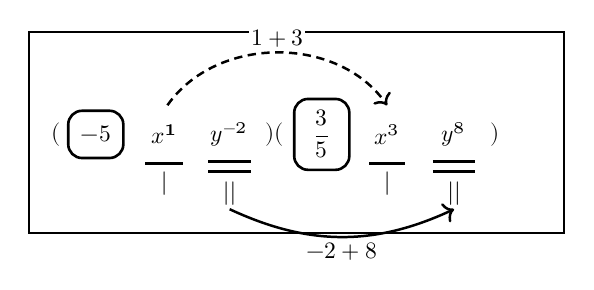
\begin{tikzpicture}[x=1cm, y=1cm, every node/.style={font=\fontsize{8.5pt}{10.5pt}\selectfont, text=black}]
        \draw[black, line width=0.85pt, fill=white] (0,0) rectangle (6.80, 2.55);
        % Expression elements spaced cleanly
        \node (lp) at (0.35, 1.25) {$($};
        \node (c1) at (0.85, 1.25) {$-5$};
        \node (x1) at (1.72, 1.25) {$x^{\mathbf{1}}$};
        \node (y1) at (2.55, 1.25) {$y^{-2}$};
        \node (rp) at (3.12, 1.25) {$)($};
        \node (c2) at (3.72, 1.25) {$\dfrac{3}{5}$};
        \node (x2) at (4.55, 1.25) {$x^{3}$};
        \node (y2) at (5.40, 1.25) {$y^{8}$};
        \node (rrp) at (5.92, 1.25) {$)$};

        % Monochrome B&W circling on coefficients
        \draw[black, line width=0.95pt, rounded corners=5pt] (0.50, 0.95) rectangle (1.20, 1.55);
        \draw[black, line width=0.95pt, rounded corners=5pt] (3.37, 0.80) rectangle (4.07, 1.70);

        % Single bar | under x & double bar || under y
        \draw[black, line width=1.1pt] (1.48, 0.88) -- (1.96, 0.88);
        \draw[black, line width=1.1pt] (4.32, 0.88) -- (4.78, 0.88);
        \node at (1.72, 0.62) {\en{|}};
        \node at (4.55, 0.62) {\en{|}};

        \draw[black, line width=1.1pt] (2.28, 0.90) -- (2.82, 0.90);
        \draw[black, line width=1.1pt] (2.28, 0.78) -- (2.82, 0.78);
        \draw[black, line width=1.1pt] (5.13, 0.90) -- (5.67, 0.90);
        \draw[black, line width=1.1pt] (5.13, 0.78) -- (5.67, 0.78);
        \node at (2.55, 0.50) {\en{||}};
        \node at (5.40, 0.50) {\en{||}};

        % Separated overhead arc for x (1+3) & under/high arc for y (-2+8) — ZERO overlap!
        \draw[black, densely dashed, line width=0.9pt, ->] (1.76, 1.62) to[out=55, in=125] node[above=1pt, fill=white, inner sep=0.6pt] {$1+3$} (4.55, 1.62);
        \draw[black, line width=0.9pt, ->] (2.55, 0.30) to[out=-25, in=-155] node[below=1pt, fill=white, inner sep=0.6pt] {$-2+8$} (5.40, 0.30);
      \end{tikzpicture}
      \end{center}
    \end{tcolorbox}

    \begin{tcolorbox}[enhanced, sharp corners, colback=white, colframe=black, boxrule=0.8pt, boxsep=1pt, top=5pt, bottom=5pt, left=5pt, right=5pt]
      \raggedright\fontsize{7.55pt}{10.8pt}\selectfont
      \textbf{ជំហាន ៣៖ ពិនិត្យក្រោយ (\en{EIA Looking-Back} ៣០ វិនាទី)៖}\\[2pt]
      \textbf{១)} តើសញ្ញាដកមុខ $-5$ បាត់ឬនៅ? \chkbox~រក្សាទុក ($\rightarrow -35, -3$)\\[1.5pt]
      \textbf{២)} ហេតុអ្វី $x\cdot x^3 = x^4$ មិនមែន $x^3$? ($x=x^{\mathbf{1}}$, \cnum{3})\\[1.5pt]
      \textbf{៣)} តើ $y^{-2}\cdot y^8$ បូក ឬគុណនិទស្សន្ត? ($-2+8=6$, ហាមគុណ!)
    \end{tcolorbox}
  \end{minipage}\hfill
  \begin{minipage}[t]{10.20cm}
    \vspace{0pt}
    \begin{tcolorbox}[enhanced, sharp corners, colback=white, colframe=black, boxrule=0.85pt, boxsep=1pt, top=6pt, bottom=6pt, left=6pt, right=6pt]
      \raggedright\fontsize{8.1pt}{12.2pt}\selectfont
      \textbf{ជំហាន ២៖ អនុវត្តដោះស្រាយ លំហាត់គំរូ ទំ.១៥ (គូស \en{[tracing]} + សំអាង \cnum{1}--\cnum{5})៖}\\[5pt]

      \textbf{ក.} គណនា $10^{-3} \times 10^4$ \quad \textit{(សម្គាល់គោលដូចគ្នា $10$, \cnum{1}, \cnum{2})}៖\\[3pt]
      $\Rightarrow 10^{-3} \times 10^4 = 10^{\,\expbox + \expbox} = 10^{\,\expbox} = \underline{\hspace{0.95cm}}$ \hfill \chkbox\ (\blankcnum)\\[7pt]

      \hrule height 0.4pt \vspace{6pt}

      \textbf{ខ.} គណនា $(-5y^2)(7y^8)$ \quad \textit{(ព័ទ្ធ \circbox{-5}, \circbox{7} និងគូស \en{||} ក្រោម $y$, \cnum{4})}៖\\[3pt]
      $\Rightarrow (\underline{\hspace{0.65cm}} \times \underline{\hspace{0.65cm}})\left(y^{\,\expbox} \cdot y^{\,\expbox}\right) = \underline{\hspace{0.80cm}} \cdot y^{\,\expbox+\expbox} = \underline{\hspace{1.15cm}}$ \hfill \mbox{\chkbox\ (\blankcnum, \blankcnum)}\\[7pt]

      \hrule height 0.4pt \vspace{6pt}

      \textbf{គ.} គណនា $\left(-5xy^{-2}\right)\left(\dfrac{3}{5}x^3 y^8\right)$ \quad \textit{(សម្រាប់ $x \neq 0,\; y \neq 0$)}៖\\[3pt]
      $\bullet$ សម្គាល់និទស្សន្តលាក់ \cnum{3}៖ $x = x^{\,\expbox}$ និងព័ទ្ធ \circbox{-5}, \circbox{\tfrac{3}{5}}\\[3pt]
      $\bullet$ ផ្ដុំមេគុណនិងគោលដូចគ្នា (\cnum{4})៖\\[3pt]
      $= \left(\underline{\hspace{0.70cm}} \times \underline{\hspace{0.70cm}}\right)\left(x^{\,\expbox} \cdot x^{\,\expbox}\right)\left(y^{\,\expbox} \cdot y^{\,\expbox}\right)$\\[4pt]
      $= \underline{\hspace{0.85cm}} \cdot x^{\,\expbox} \cdot y^{\,\expbox} = \underline{\hspace{1.85cm}}$ \hfill \chkbox\ (\blankcnum, \blankcnum, \blankcnum)
    \end{tcolorbox}
    \vspace{5pt}
    \begin{tcolorbox}[enhanced, sharp corners, colback=panelgray, colframe=black, boxrule=0.75pt, boxsep=1pt, top=4pt, bottom=4pt, left=5pt, right=5pt]
      \raggedright\fontsize{7.2pt}{10.2pt}\selectfont
      \textbf{ធនាគារ \cnum{1}--\cnum{5}៖} \cnum{1} គោលដូចគ្នា \en{|} \cnum{2} $a^m\cdot a^n=a^{m+n}$ ($a\neq 0$) \en{|} \cnum{3} លាក់ $1$ \& វង់ក្រចក \en{|} \cnum{4} ផ្ដុំមេគុណ-អញ្ញាត \en{|} \cnum{5} ស្ពាន $a^{-n}, a^0$
    \end{tcolorbox}
  \end{minipage}
\end{tcolorbox}%
}

\vspace{4pt}
\eFourCardEXPMUL{ប័ណ្ណទី ១}

\vspace{12pt}
\noindent\scissors\ \dotfill\ \textbf{កាត់តាមស្នាមចុចចែកជា ២ ប័ណ្ណ (\en{Cut Along Dashed Line})} \dotfill\ \scissors
\vspace{12pt}

\eFourCardEXPMUL{ប័ណ្ណទី ២}

\clearpage

% ============================================================================
% ទំព័រទី ៣៖ E5 Evaluate — តារាង Relay ៣ តួនាទី (ប្រតិបត្តិ ទំ.១៥ ក, ខ, គ + Erratum #1 + បិទ E1)
% ============================================================================
\pagebanner{សម្ភារៈទី ៣៖ សន្លឹក \enbf{Relay} ៣ តួនាទី «ប្រតិបត្តិ» \enbf{(}ទំ.១៥ \enbf{\&} កែពុម្ព\enbf{)} និងបិទ \enbf{E1}}{ទំព័រ ៣/៦ \en{-- E5 Evaluate} (កាត់ ២ សន្លឹក \scissors)}

\newcommand{\eFiveSheetEXPMUL}[1]{%
\begin{tcolorbox}[
  enhanced, sharp corners, colback=white, colframe=white,
  borderline={1.0pt}{0pt}{black, dashed},
  boxsep=1pt, top=10pt, bottom=10pt, left=5.5pt, right=5.5pt
]
  \begin{tcolorbox}[
    enhanced, sharp corners, colback=headgray, colframe=black,
    boxrule=0.85pt, boxsep=1pt, top=4.5pt, bottom=4.5pt, left=5.5pt, right=5.5pt, after skip=6pt
  ]
    \fontsize{8.1pt}{11.4pt}\selectfont
    \textbf{\scissors\ សន្លឹក \en{Relay} ៣ តួនាទី (#1) \en{--} ប្រតិបត្តិ (ទំ.១៥)} \hfill ក្រុម៖ $\underline{\hspace{2.6cm}}$\\[3pt]
    \textbf{ប្រធាន៖} សម្រួល៖ \textbf{ក.} $x^9 \cdot x^4$ \quad \textbf{ខ.} $\left(-\dfrac{3}{2}\right)^2 \cdot \left(-\dfrac{3}{2}\right)^{-2}$ \quad \textbf{គ. [កែពុម្ព \en{Erratum \#1}]៖} $(3x^4 y^{-3})\left(-\dfrac{4}{3}x^{-2}y\right)$ \textit{(ជំនួសពុម្ពខុស $x^{-2y}$; $x,y\neq 0$)}
  \end{tcolorbox}

  \renewcommand{\arraystretch}{1.24}
  {\centering\setlength{\tabcolsep}{4pt}%
  \begin{tabular}{|L{5.65cm}|L{6.55cm}|L{5.30cm}|}
    \hline
    \cellcolor{panelgray}\centering\arraybackslash\fontsize{8.0pt}{10.8pt}\selectfont\textbf{តួនាទី ១៖ អ្នកគូស \en{[tracing]} \en{\& Pause-Ask!}}\newline {\fontsize{7.2pt}{9.8pt}\selectfont ព័ទ្ធមេគុណ គូស \en{|}, \en{||}, កត់និទស្សន្តលាក់ \en{1}} &
    \cellcolor{panelgray}\centering\arraybackslash\fontsize{8.0pt}{10.8pt}\selectfont\textbf{តួនាទី ២៖ អ្នកគណនា និងសំអាង \cnum{1}--\cnum{5}}\newline {\fontsize{7.2pt}{9.8pt}\selectfont អនុវត្ត $a^m\cdot a^n = a^{m+n}$ និងដាក់លេខ \cnum{1}--\cnum{5}} &
    \cellcolor{panelgray}\centering\arraybackslash\fontsize{8.0pt}{10.8pt}\selectfont\textbf{តួនាទី ៣៖ អ្នកពិនិត្យសញ្ញា \en{\&} បិទ \en{E1}}\newline {\fontsize{7.2pt}{9.8pt}\selectfont \en{Pause-Review!} \en{\&} បិទបេសកកម្ម \en{Server E1}} \\ \hline

    % --- Column 1: Visual Marker + Pause-Ask! ---
    \fontsize{7.9pt}{11.4pt}\selectfont
    \textbf{គូសដាន \en{[tracing]} លើ \textbf{ក, ខ, គ}៖}\par\vspace{4pt}
    $\bullet$ \textbf{ក.} គោលដូចគ្នា $x$៖ \chkbox~សម្គាល់ \en{|} ក្រោម $x^9, x^4$\par\vspace{4pt}
    $\bullet$ \textbf{ខ.} គោលប្រភាគអវិជ្ជមាន៖\par
    \chkbox~រក្សាវង់ក្រចក $\left(-\frac{3}{2}\right)$ ទាំងពីរតួ!\par\vspace{4pt}
    $\bullet$ \textbf{គ. (កែពុម្ព \en{Erratum \#1})៖}\par
    $(3x^4 y^{-3})\left(-\dfrac{4}{3}x^{-2}y^{\,\expbox}\right)$\par\vspace{3pt}
    \chkbox~ព័ទ្ធ \circbox{3}, \circbox{-\frac{4}{3}} \en{|} \chkbox~គូស \en{|} ក្រោម $x$ \en{|} \chkbox~គូស \en{||} ក្រោម $y$ \par\vspace{7pt}
    \begin{tcolorbox}[enhanced, sharp corners, colback=panelgray, colframe=black, boxrule=0.75pt, boxsep=1pt, top=4.5pt, bottom=4.5pt, left=5pt, right=5pt]
      \raggedright\fontsize{7.4pt}{10.6pt}\selectfont
      \chkbox\ \textbf{\en{Pause-Ask!}} ហេតុអ្វីកែ $x^{-2y} \to x^{-2}y^1$ ហើយហេតុអ្វី $y$ មាននិទស្សន្ត \textbf{១} (\cnum{3})?
    \end{tcolorbox}
    &
    % --- Column 2: Calculator & Warrant 1-5 ---
    \fontsize{7.9pt}{11.8pt}\selectfont
    \textbf{ក.} $x^9 \cdot x^4 = x^{\,\expbox+\expbox} = \underline{\hspace{1.05cm}}$ \hfill (\blankcnum)\par\vspace{6pt}
    \textbf{ខ.} $\left(-\dfrac{3}{2}\right)^2 \cdot \left(-\dfrac{3}{2}\right)^{-2} = \left(-\dfrac{3}{2}\right)^{\,\expbox+\expbox}$\par\vspace{3pt}
    $= \left(-\dfrac{3}{2}\right)^{\,\expbox} = \underline{\hspace{0.85cm}}$ \hfill (\blankcnum, \blankcnum)\par\vspace{6pt}
    \textbf{គ.} $(3x^4 y^{-3})\left(-\dfrac{4}{3}x^{-2}y\right)$\par\vspace{3pt}
    $= \left(\underline{\hspace{0.50cm}}\times \underline{\hspace{0.65cm}}\right)\left(x^{\,\expbox}\cdot x^{\,\expbox}\right)\left(y^{\,\expbox}\cdot y^{\,\expbox}\right)$\par\vspace{3pt}
    $= \underline{\hspace{0.80cm}}x^{\,\expbox}y^{\,\expbox}$ \hfill (\blankcnum, \blankcnum, \blankcnum)\par\vspace{7pt}
    \begin{tcolorbox}[enhanced, sharp corners, colback=panelgray, colframe=black, boxrule=0.7pt, boxsep=1pt, top=3.5pt, bottom=3.5pt, left=4.5pt, right=4.5pt]
      \raggedright\fontsize{7.2pt}{10.2pt}\selectfont
      \textbf{សំអាង៖} \cnum{1} គោលដូច \en{|} \cnum{2} $a^{m+n}$ \en{|} \cnum{3} លាក់ $1$ \en{|} \cnum{4} ផ្ដុំ \en{|} \cnum{5} $a^0=1$
    \end{tcolorbox}
    &
    % --- Column 3: Sign Checker Pause-Review! & E1 Closure ---
    \fontsize{7.7pt}{11.2pt}\selectfont
    \chkbox\ \textbf{\en{Pause-Review!}} ផ្ទៀងសញ្ញា \en{\&} សំអាង៖\par\vspace{4.5pt}
    \chkbox~១) តើ $3\times\left(-\frac{4}{3}\right) = -4$ (មិនភ្លេចសញ្ញាដក)?\par\vspace{4.5pt}
    \chkbox~២) តើ $y^{-3}\cdot y^1 = y^{-2}$ (មិនមែន $y^{-3}$ ឬ $y^3$)?\par\vspace{4.5pt}
    \chkbox~៣) តើ $\left(-\frac{3}{2}\right)^0 = +1$ (មិនមែន $0$ ឬ $-1$)?\par\vspace{9pt}
    \begin{tcolorbox}[enhanced, sharp corners, colback=panelgray, colframe=black, boxrule=0.8pt, boxsep=1pt, top=6pt, bottom=6pt, left=5pt, right=5pt]
      \raggedright\fontsize{7.6pt}{11.2pt}\selectfont
      \textbf{បិទបេសកកម្ម \en{E1 (Server Library)}៖}\\[3pt]
      $\bullet$ វីដេអូសរុប៖ $2^3 \times 2^4 = 2^{\,\expbox} = \underline{\hspace{0.72cm}}$ វីដេអូ\\[3pt]
      $\bullet$ ទំហំទិន្នន័យ៖ $10^{-3}\times 10^4 = 10^{\,\expbox} = \underline{\hspace{0.72cm}}\unit{MB}$\\[3pt]
      $\Rightarrow$ ដំណោះស្រាយ៖ ទុកគោល បូកនិទស្សន្ត!
    \end{tcolorbox}
    \\ \hline
  \end{tabular}\par}
\end{tcolorbox}%
}

\vspace{6pt}
\eFiveSheetEXPMUL{សន្លឹកទី ១}

\vspace{18pt}
\noindent\scissors\ \dotfill\ \textbf{កាត់តាមស្នាមចុចចែកជា ២ សន្លឹក (\en{Cut Along Dashed Line})} \dotfill\ \scissors
\vspace{18pt}

\eFiveSheetEXPMUL{សន្លឹកទី ២}

\clearpage

% ============================================================================
% ទំព័រទី ៤៖ ផ្ទាំងសំអាងគោល ២.២ — ធនាគារហេតុផល ①–⑤ & ប្រអប់ព្រមានដែនវង់ក្រចក
% ============================================================================
\begin{tcolorbox}[
  enhanced, sharp corners, colback=white, colframe=black,
  boxrule=1.5pt, borderline={0.6pt}{2.2pt}{black},
  boxsep=1pt, top=18pt, bottom=18pt, left=8pt, right=8pt
]
  \begin{center}
    {\fontsize{8.8pt}{12.0pt}\selectfont មន្ទីរអប់រំ យុវជន និងកីឡា ខេត្តកំពង់ធំ \en{|} ការិយាល័យអប់រំ យុវជន និងកីឡា ស្រុកកំពង់ស្វាយ \en{|} អនុវិទ្យាល័យព្រះក្រសាំង}\\[4pt]
    {\muol\fontsize{12.6pt}{18.0pt}\selectfont ផ្ទាំងសំអាងគោល ២\enbf{.}២៖ វិធីគុណស្វ័យគុណមាននិទស្សន្តរ៉ឺឡាទីប \enbf{(}\mbox{\normalfont\fontsize{13pt}{15pt}\selectfont\ding{182}}\enbf{--}\mbox{\normalfont\fontsize{13pt}{15pt}\selectfont\ding{186}}\enbf{)}}\\[4pt]
    {\fontsize{8.3pt}{11.5pt}\selectfont គណិតវិទ្យា ថ្នាក់ទី៨ \en{--} មេរៀនទី២ (ទំ.១៥\en{--}១៦, ២៥) \en{|} គ្រូបង្រៀន៖ ហុក ប៊ុនថែន \en{|} ថ្ងៃចន្ទ ៧កើត កត្តិក ព.ស. ២៥៧០ (ថ្ងៃទី១៦ ខែវិច្ឆិកា ឆ្នាំ២០២៦)}\\[5pt]
    \khmflourish
  \end{center}
  \vspace{15pt}

  % --- ផ្នែកទី ១៖ ប្រអប់ "ជាទូទៅ" កែ Erratum #2 (ឆ្វេង) & Sign-Scope Warning Box (ស្ដាំ) ---
  \noindent
  \begin{minipage}[t]{8.90cm}
    \begin{tcolorbox}[enhanced, sharp corners, colback=white, colframe=black, boxrule=0.95pt, boxsep=1pt, equal height group=posterTopEXP, top=9pt, bottom=9pt, left=6.5pt, right=6.5pt]
      \raggedright\fontsize{8.7pt}{12.8pt}\selectfont
      \textbf{វិធានទូទៅ (កែតម្រូវប្រអប់ «ជាទូទៅ» ទំ.១៥ \en{-- Erratum \#2})៖}\\[4pt]
      បើ $a$ ជាចំនួនសនិទាន ($a \neq 0$ កាលណា $m \le 0$ ឬ $n \le 0$) និង $m, n \in \mathbb{Z}$ ជាចំនួនគត់រ៉ឺឡាទីប នោះ៖
      \[
        a^m \cdot a^n = a^{m+n}
      \]
      \textbf{ឧទាហរណ៍គោល (ទំ.១៥)៖}\\[2pt]
      \textbf{ក.} $2^3\times 2^4 = 2^{3+4} = 2^7$ \quad \textbf{ខ.} $3^5\times 3^7 = 3^{5+7} = 3^{12}$\\[3pt]
      \textbf{គ.} $\left(\frac{3}{2}\right)^2\cdot\left(\frac{3}{2}\right)^3 = \left(\frac{3}{2}\right)^{2+3} = \left(\frac{3}{2}\right)^5$ \quad \textbf{ឃ.} $a^m\cdot a^n = a^{m+n}$
    \end{tcolorbox}
  \end{minipage}\hfill
  \begin{minipage}[t]{8.60cm}
    \begin{tcolorbox}[enhanced, sharp corners, colback=panelgray, colframe=black, boxrule=0.95pt, boxsep=1pt, equal height group=posterTopEXP, top=9pt, bottom=9pt, left=6.5pt, right=6.5pt]
      \raggedright\fontsize{8.7pt}{12.5pt}\selectfont
      \textbf{\ding{45}\ ប្រអប់ព្រមានដែនវង់ក្រចក \en{(Sign-Scope Warning)}៖}\\[5pt]
      \begin{center}
      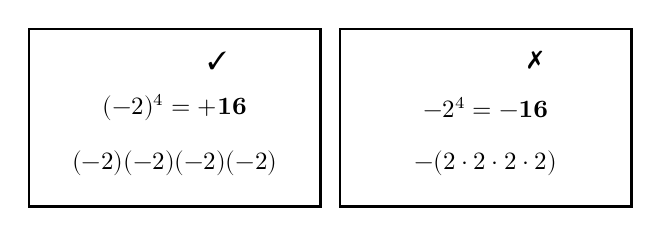
\begin{tikzpicture}[x=1cm, y=1cm, every node/.style={font=\fontsize{9.0pt}{11.0pt}\selectfont, text=black}]
        \draw[black, line width=1.0pt, fill=white] (0, 0) rectangle (3.70, 2.25);
        \node at (1.85, 1.85) {\textbf{មានវង់ក្រចក} \ding{51}};
        \node at (1.85, 1.25) {$(-2)^4 = \mathbf{+16}$};
        \node at (1.85, 0.55) {$(-2)(-2)(-2)(-2)$};

        \draw[black, line width=1.0pt, fill=white] (3.95, 0) rectangle (7.65, 2.25);
        \node at (5.80, 1.85) {\textbf{គ្មានវង់ក្រចក} \ding{55}};
        \node at (5.80, 1.25) {$-2^4 = \mathbf{-16}$};
        \node at (5.80, 0.55) {$-(2\cdot 2\cdot 2\cdot 2)$};
      \end{tikzpicture}
      \end{center}
      \vspace{4pt}
      $\bullet$ \textbf{ចងចាំ៖} $(-3)^0 = +1$ ប៉ុន្តែ $-3^0 = -1$ ($a\neq 0$)!
    \end{tcolorbox}
  \end{minipage}

  \vspace{16pt}

  % --- ផ្នែកទី ២៖ តារាងធនាគារហេតុផល ①–⑤ (Print-Safe B&W) ---
  \fontsize{8.8pt}{12.8pt}\selectfont
  \renewcommand{\arraystretch}{1.82}
  \begin{tabular}{|C{0.72cm}|L{3.95cm}|L{6.30cm}|C{5.00cm}|}
    \hline
    \cellcolor{headgray}\textbf{លេខ} &
    \cellcolor{headgray}\centering\arraybackslash\textbf{ឈ្មោះវិធាន / លក្ខខណ្ឌ} &
    \cellcolor{headgray}\centering\arraybackslash\textbf{និមិត្តសញ្ញា និងរបៀបអនុវត្ត} &
    \cellcolor{headgray}\centering\arraybackslash\textbf{រូបសម្គាល់ ស-ខ្មៅ} \\ \hline

    \cnum{1} &
    \textbf{ច្រកគោលដូចគ្នា}\newline (\en{Same-Base Gate}) &
    ពិនិត្យថា\textbf{គោលដូចគ្នា}មុនបូកនិទស្សន្ត។ \textbf{ហាម} គុណ ឬបូកគោល ($2^3\cdot 2^4\neq 4^7$, $2^3\cdot 3^2\neq 6^5$)~។ &
    \raisebox{-0.35\height}{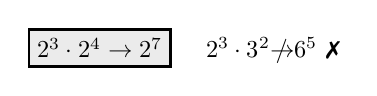
\begin{tikzpicture}[x=1cm, y=1cm, every node/.style={font=\fontsize{8.8pt}{11pt}\selectfont, text=black}]
      \node[draw=black, line width=0.95pt, fill=panelgray, inner sep=3pt] at (0.85, 0.50) {$2^3 \cdot 2^4 \to 2^7$};
      \node at (3.05, 0.50) {$2^3\cdot 3^2 \not\to 6^5$ \ding{55}};
    \end{tikzpicture}} \\ \hline

    \cnum{2} &
    \textbf{វិធានគុណស្វ័យគុណគោលដូចគ្នា} &
    $a^m \cdot a^n = a^{m+n}$ ($m,n\in\mathbb{Z}$; ត្រូវមាន \textbf{$a \neq 0$} កាលណា $m\le 0$ ឬ $n\le 0$)។ \textbf{ហាម} គុណនិទស្សន្ត~។ &
    \raisebox{-0.35\height}{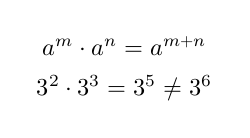
\begin{tikzpicture}[x=1cm, y=1cm, every node/.style={font=\fontsize{8.8pt}{11pt}\selectfont, text=black}]
      \node at (1.50, 0.65) {$a^m \cdot a^n = a^{m+n}$};
      \node at (1.50, 0.12) {$3^2\cdot 3^3 = 3^5 \neq 3^6$};
    \end{tikzpicture}} \\ \hline

    \cnum{3} &
    \textbf{និទស្សន្តលាក់ \en{1} \& ដែនវង់ក្រចក} &
    $x=x^{\mathbf{1}},\; y=y^{\mathbf{1}},\; 2=2^{\mathbf{1}},\; -x^7=(-1)x^7$ និងញែក $(-a)^n$ ពី $-a^n$~។ &
    \raisebox{-0.35\height}{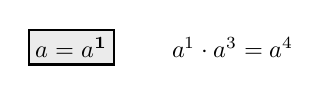
\begin{tikzpicture}[x=1cm, y=1cm, every node/.style={font=\fontsize{8.8pt}{11pt}\selectfont, text=black}]
      \node[draw=black, line width=0.9pt, fill=panelgray, inner sep=2.5pt] at (0.80, 0.45) {$a = a^{\mathbf{1}}$};
      \node at (2.85, 0.45) {$a^1\cdot a^3 = a^4$};
    \end{tikzpicture}} \\ \hline

    \cnum{4} &
    \textbf{ផ្ដុំមេគុណលេខ \& គោលអញ្ញាតដូចគ្នា} &
    \en{[tracing]}៖ \textbf{ព័ទ្ធរង្វង់}មេគុណ គុណមេគុណ $\cdot$ គូស \en{|} ក្រោម $x$, \en{||} ក្រោម $y$ រួចគូសធ្នូបូកនិទស្សន្ត~។ &
    \raisebox{-0.35\height}{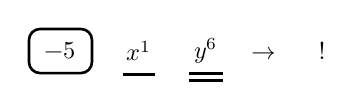
\begin{tikzpicture}[x=1cm, y=1cm, every node/.style={font=\fontsize{8.8pt}{11pt}\selectfont, text=black}]
      \draw[black, line width=0.95pt, rounded corners=4pt] (0.05,0.22) rectangle (0.85,0.78);
      \node at (0.45, 0.50) {$-5$};
      \node at (1.45, 0.50) {$x^1$};
      \draw[black, line width=1.1pt] (1.25, 0.20)--(1.65, 0.20);
      \node at (2.30, 0.50) {$y^6$};
      \draw[black, line width=1.1pt] (2.08, 0.22)--(2.52, 0.22) (2.08, 0.12)--(2.52, 0.12);
      \node at (3.35, 0.50) {$\to$ ផ្ដុំ!};
    \end{tikzpicture}} \\ \hline

    \cnum{5} &
    \textbf{ស្ពាននិទស្សន្តអវិជ្ជមាន និងសូន្យ} &
    $a^{-n} = \dfrac{1}{a^n}$ និង $a^0 = 1$ ($a\neq 0$) រួមទាំងបន្សាបគូសូន្យ $a^k\cdot a^{-k}=a^0=1$~។ &
    \raisebox{-0.35\height}{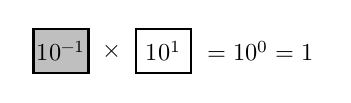
\begin{tikzpicture}[x=1cm, y=1cm, every node/.style={font=\fontsize{8.8pt}{11pt}\selectfont, text=black}]
      \fill[midgray] (0.10,0.22) rectangle (0.80,0.78);
      \draw[black, line width=0.95pt] (0.10,0.22) rectangle (0.80,0.78);
      \node at (0.45, 0.50) {$10^{-1}$};
      \node at (1.10, 0.50) {$\times$};
      \draw[black, line width=0.95pt, fill=white] (1.40,0.22) rectangle (2.10,0.78);
      \node at (1.75, 0.50) {$10^{1}$};
      \node at (2.98, 0.50) {$= 10^0 = 1$};
    \end{tikzpicture}} \\ \hline
  \end{tabular}

  \vspace{12pt}

  % --- ផ្នែកទី ៣៖ កំណែពុម្ពសៀវភៅ MoEYS (ឆ្វេង) & ស្ពានត្រៀមមេរៀន ២.៣ (ស្ដាំ) ---
  \noindent
  \begin{minipage}[t]{8.75cm}
    \begin{tcolorbox}[
      enhanced, sharp corners, colback=white, colframe=black,
      boxrule=1.05pt, boxsep=1pt, equal height group=posterBotEXP,
      top=8pt, bottom=8pt, left=6pt, right=6pt,
      title={\textbf{កំណែពុម្ពសៀវភៅគោល (\en{MoEYS pp. 15, 25 Errata})}},
      colbacktitle=headgray, coltitle=black, fonttitle=\fontsize{8.8pt}{12.0pt}\selectfont
    ]
      \raggedright\fontsize{8.5pt}{12.4pt}\selectfont
      \textbf{១) \en{Erratum \#1} (ប្រតិបត្តិ គ. ទំ.១៥)៖} កែពុម្ព $x^{-2y} \to \mathbf{x^{-2}y}$៖\\
      $\quad (3x^4 y^{-3})\left(-\frac{4}{3}x^{-2}y\right) = -4x^2y^{-2}$ ($x\neq 0, y\neq 0$)។\\[5pt]
      \textbf{២) \en{Erratum \#2} (ទំ.១៥)៖} បន្ថែម $a\neq 0$ និងស្ពាន $a^0=1, a^{-n}=\frac{1}{a^n}$។\\[5pt]
      \textbf{៣) ទំ.២៥ \en{\#7} ក៖} ជៀសវាង \en{\#7} ក ដែលបោះពុម្ពខ្វះតួគុណទី ២!
    \end{tcolorbox}
  \end{minipage}\hfill
  \begin{minipage}[t]{8.75cm}
    \begin{tcolorbox}[
      enhanced, sharp corners, colback=white, colframe=black,
      boxrule=1.05pt, boxsep=1pt, equal height group=posterBotEXP,
      top=8pt, bottom=8pt, left=6pt, right=6pt,
      title={\textbf{ស្ពានភ្ជាប់មេរៀន ២.៣៖ វិធីចែកស្វ័យគុណ (ទំ.១៦)}},
      colbacktitle=midgray, coltitle=black, fonttitle=\fontsize{8.8pt}{12.0pt}\selectfont
    ]
      \centering
      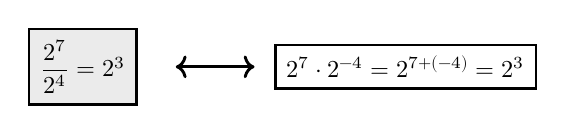
\begin{tikzpicture}[x=1cm, y=1cm, every node/.style={font=\fontsize{8.8pt}{11.0pt}\selectfont, text=black}]
        \node[draw=black, line width=0.95pt, fill=panelgray, inner sep=4pt] (d1) at (1.50, 0.65) {$\dfrac{2^7}{2^4} = 2^3$};
        \draw[black, line width=1.05pt, <->] (2.68, 0.65) -- (3.68, 0.65);
        \node[draw=black, line width=0.95pt, fill=white, inner sep=4pt] (d2) at (5.60, 0.65) {$2^7 \cdot 2^{-4} = 2^{7+(-4)} = 2^3$};
      \end{tikzpicture}
      \par\vspace{7pt}\raggedright\fontsize{8.5pt}{12.4pt}\selectfont
      $\bullet$ \textbf{គន្លឹះភ្ជាប់មេរៀនបន្ទាប់៖} ការចែកនឹង $a^n$ ($a\neq 0$) គឺស្មើនឹងការគុណនឹង $a^{-n}$ តាមវិធាន \cnum{2} និង \cnum{5} ដដែល!
    \end{tcolorbox}
  \end{minipage}
  \par\vspace{14pt}
  \begin{tcolorbox}[enhanced, sharp corners, colback=panelgray, colframe=black, boxrule=0.8pt, boxsep=1pt, top=8pt, bottom=8pt, left=7pt, right=7pt]
    \centering\fontsize{8.6pt}{12.2pt}\selectfont
    \textbf{គោលការណ៍ប្រើផ្ទាំងសំអាងក្នុងថ្នាក់ (\en{E3--E5})៖} រាល់ជំហានដោះស្រាយក្នុង \textbf{លំហាត់គំរូ (ទំ.១៥)}, \textbf{ប្រតិបត្តិ (ទំ.១៥)} និង \textbf{លំហាត់ \en{\#6--\#7} (ទំ.២៥)} ត្រូវចុះលេខសំអាង \cnum{1}--\cnum{5} ភ្ជាប់ជានិច្ច!
  \end{tcolorbox}
\end{tcolorbox}

\clearpage

% ============================================================================
% ទំព័រទី ៥៖ កាតវិនិច្ឆ័យរហ័ស "កាត A–D" + ចម្លើយគ្រូ + សំបុត្រចេញ ៣ សំណួរ (E5 Evaluate)
% ============================================================================
\pagebanner{សម្ភារៈទី ៥៖ កាតវិនិច្ឆ័យរហ័ស «កាត \enbf{A--D}» \enbf{\&} សំបុត្រចេញរហ័ស \enbf{E5}}{ទំព័រ ៥/៦ \en{-- E5 Evaluate}}

{\fontsize{8.3pt}{11.6pt}\selectfont
\textbf{វិធីលេងក្នុងថ្នាក់៖} គ្រូលើកកាតម្ដងមួយ $\rightarrow$ សិស្សផ្ទៀងតាមធនាគារ \cnum{1}--\cnum{5} $\rightarrow$ លើក \textbf{មេដៃឡើង (ត្រឹមត្រូវ \ding{51})} ឬ \textbf{ខ្វែងដៃ (ខុស/អន្ទាក់ \ding{55})} + បង្ហាញម្រាមដៃ \en{1--5} ប្រាប់លេខវិធាន។}

\vspace{7pt}

% --- ជួរទី ១៖ កាត A & កាត B ---
\noindent
\begin{tcolorbox}[
  enhanced, sharp corners, colback=white, colframe=white,
  borderline={1.0pt}{0pt}{black, dashed},
  width=9.25cm, equal height group=expfoilrow1, nobeforeafter,
  boxsep=1pt, top=7pt, bottom=7pt, left=6pt, right=6pt
]
  \noindent\colorbox{black}{\textcolor{white}{\Large\textbf{\en{ A }}}}\hspace{0.22cm}{\fontsize{9.1pt}{12.5pt}\selectfont\textbf{កាត \en{A} ៖ ពិនិត្យគោល និងនិទស្សន្ត}}\par\vspace{6pt}
  \begin{center}
  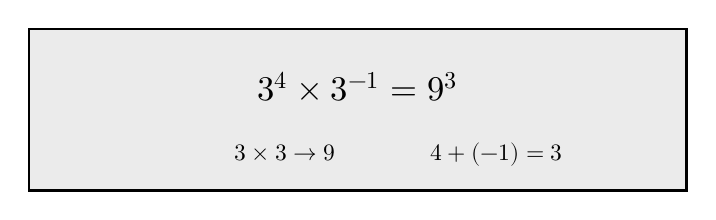
\begin{tikzpicture}[x=1cm, y=1cm, every node/.style={font=\fontsize{8.5pt}{10.5pt}\selectfont, text=black}]
    \draw[black, line width=1.0pt, fill=panelgray] (0, 0) rectangle (8.35, 2.05);
    \node[font=\fontsize{12.5pt}{15pt}\selectfont] at (4.175, 1.32) {$3^4 \times 3^{-1} = 9^3$};
    \node at (4.175, 0.45) {សង្កេត៖ គោល $3 \times 3 \to 9$ និងនិទស្សន្ត $4+(-1)=3$};
  \end{tikzpicture}
  \end{center}
  \vspace{3pt}
  {\centering\fontsize{8.4pt}{11.6pt}\selectfont គេអះអាងថា $3^4 \times 3^{-1} = 9^3$ ។\par}
  \vfill
  \begin{tcolorbox}[enhanced, sharp corners, colback=panelgray, colframe=black, boxrule=0.8pt, boxsep=1pt, top=4.5pt, bottom=4.5pt, left=4pt, right=4pt]
    \centering\fontsize{8.8pt}{12.0pt}\selectfont
    \textbf{សំណួរ៖} ត្រឹមត្រូវឬទេ? \quad \chkbox~ពិត (\ding{51}) \quad \chkbox~ខុស (\ding{55})
  \end{tcolorbox}
\end{tcolorbox}%
\hfill
\begin{tcolorbox}[
  enhanced, sharp corners, colback=white, colframe=white,
  borderline={1.0pt}{0pt}{black, dashed},
  width=9.25cm, equal height group=expfoilrow1, nobeforeafter,
  boxsep=1pt, top=7pt, bottom=7pt, left=6pt, right=6pt
]
  \noindent\colorbox{black}{\textcolor{white}{\Large\textbf{\en{ B }}}}\hspace{0.22cm}{\fontsize{9.1pt}{12.5pt}\selectfont\textbf{កាត \en{B} ៖ គុណឯកធាតុមានអញ្ញាត ២}}\par\vspace{6pt}
  \begin{center}
  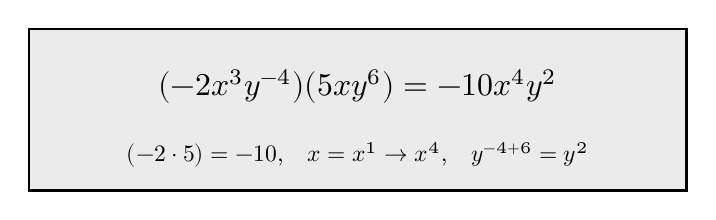
\begin{tikzpicture}[x=1cm, y=1cm, every node/.style={font=\fontsize{8.5pt}{10.5pt}\selectfont, text=black}]
    \draw[black, line width=1.0pt, fill=panelgray] (0, 0) rectangle (8.35, 2.05);
    \node[font=\fontsize{11.5pt}{14.5pt}\selectfont] at (4.175, 1.32) {$(-2x^3 y^{-4})(5xy^6) = -10x^4 y^2$};
    \node at (4.175, 0.45) {$(-2\cdot 5)=-10$,\quad $x=x^1\to x^4$,\quad $y^{-4+6}=y^2$};
  \end{tikzpicture}
  \end{center}
  \vspace{3pt}
  {\centering\fontsize{8.4pt}{11.6pt}\selectfont គេអះអាងថា $(-2x^3 y^{-4})(5xy^6) = -10x^4 y^2$ ($x,y\neq 0$)។\par}
  \vfill
  \begin{tcolorbox}[enhanced, sharp corners, colback=panelgray, colframe=black, boxrule=0.8pt, boxsep=1pt, top=4.5pt, bottom=4.5pt, left=4pt, right=4pt]
    \centering\fontsize{8.8pt}{12.0pt}\selectfont
    \textbf{សំណួរ៖} ត្រឹមត្រូវឬទេ? \quad \chkbox~ពិត (\ding{51}) \quad \chkbox~ខុស (\ding{55})
  \end{tcolorbox}
\end{tcolorbox}

\vspace{9pt}

% --- ជួរទី ២៖ កាត C & កាត D ---
\noindent
\begin{tcolorbox}[
  enhanced, sharp corners, colback=white, colframe=white,
  borderline={1.0pt}{0pt}{black, dashed},
  width=9.25cm, equal height group=expfoilrow2, nobeforeafter,
  boxsep=1pt, top=7pt, bottom=7pt, left=6pt, right=6pt
]
  \noindent\colorbox{black}{\textcolor{white}{\Large\textbf{\en{ C }}}}\hspace{0.22cm}{\fontsize{9.1pt}{12.5pt}\selectfont\textbf{កាត \en{C} ៖ ស្វ័យគុណ ៣ តួ និងលាក់ \en{1}}}\par\vspace{6pt}
  \begin{center}
  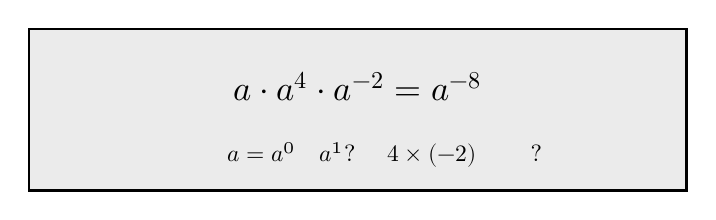
\begin{tikzpicture}[x=1cm, y=1cm, every node/.style={font=\fontsize{8.5pt}{10.5pt}\selectfont, text=black}]
    \draw[black, line width=1.0pt, fill=panelgray] (0, 0) rectangle (8.35, 2.05);
    \node[font=\fontsize{12.5pt}{15pt}\selectfont] at (4.175, 1.32) {$a \cdot a^4 \cdot a^{-2} = a^{-8}$};
    \node at (4.175, 0.45) {សង្កេត៖ $a=a^0$ ឬ $a^1$? តើ $4\times(-2)$ ត្រូវទេ?};
  \end{tikzpicture}
  \end{center}
  \vspace{3pt}
  {\centering\fontsize{8.4pt}{11.6pt}\selectfont គេអះអាងថា $a \cdot a^4 \cdot a^{-2} = a^{-8}$ ($a\neq 0$)។\par}
  \vfill
  \begin{tcolorbox}[enhanced, sharp corners, colback=panelgray, colframe=black, boxrule=0.8pt, boxsep=1pt, top=4.5pt, bottom=4.5pt, left=4pt, right=4pt]
    \centering\fontsize{8.8pt}{12.0pt}\selectfont
    \textbf{សំណួរ៖} ត្រឹមត្រូវឬទេ? \quad \chkbox~ពិត (\ding{51}) \quad \chkbox~ខុស (\ding{55})
  \end{tcolorbox}
\end{tcolorbox}%
\hfill
\begin{tcolorbox}[
  enhanced, sharp corners, colback=white, colframe=white,
  borderline={1.0pt}{0pt}{black, dashed},
  width=9.25cm, equal height group=expfoilrow2, nobeforeafter,
  boxsep=1pt, top=7pt, bottom=7pt, left=6pt, right=6pt
]
  \noindent\colorbox{black}{\textcolor{white}{\Large\textbf{\en{ D }}}}\hspace{0.22cm}{\fontsize{9.1pt}{12.5pt}\selectfont\textbf{កាត \en{D} ៖ ដែនវង់ក្រចក និងសញ្ញាដក}}\par\vspace{6pt}
  \begin{center}
  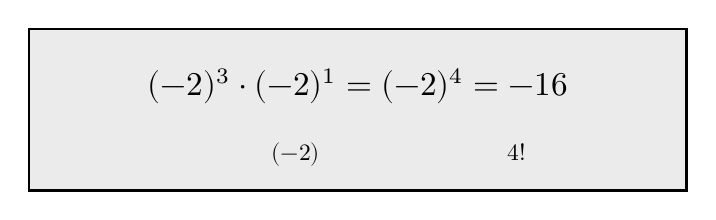
\begin{tikzpicture}[x=1cm, y=1cm, every node/.style={font=\fontsize{8.5pt}{10.5pt}\selectfont, text=black}]
    \draw[black, line width=1.0pt, fill=panelgray] (0, 0) rectangle (8.35, 2.05);
    \node[font=\fontsize{12pt}{15pt}\selectfont] at (4.175, 1.32) {$(-2)^3 \cdot (-2)^1 = (-2)^4 = -16$};
    \node at (4.175, 0.45) {សង្កេត៖ គោល $(-2)$ ក្នុងវង់ក្រចកលើកស្វ័យគុណគូ $4$!};
  \end{tikzpicture}
  \end{center}
  \vspace{3pt}
  {\centering\fontsize{8.4pt}{11.6pt}\selectfont គេអះអាងថា $(-2)^3 \cdot (-2)^1 = (-2)^4 = -16$ ។\par}
  \vfill
  \begin{tcolorbox}[enhanced, sharp corners, colback=panelgray, colframe=black, boxrule=0.8pt, boxsep=1pt, top=4.5pt, bottom=4.5pt, left=4pt, right=4pt]
    \centering\fontsize{8.8pt}{12.0pt}\selectfont
    \textbf{សំណួរ៖} ត្រឹមត្រូវឬទេ? \quad \chkbox~ពិត (\ding{51}) \quad \chkbox~ខុស (\ding{55})
  \end{tcolorbox}
\end{tcolorbox}

\vspace{10pt}

% --- ផ្នែកទី ៣៖ ចម្លើយគ្រូ (កាត A–D & Exit Ticket) + សំបុត្រចេញ ៣ សំណួរ ---
\noindent\scissors\ \dotfill\ \textbf{កាត់ទុកសម្រាប់គ្រូ (\en{Teacher Key}) \en{--} ចម្លើយកាត \en{A--D} និងសំបុត្រចេញ} \dotfill\ \scissors

\vspace{6pt}
\begin{tcolorbox}[
  enhanced, sharp corners, colback=panelgray, colframe=black,
  boxrule=0.95pt, boxsep=1pt, top=6pt, bottom=6pt, left=6pt, right=6pt
]
  \fontsize{7.8pt}{11.0pt}\selectfont
  \renewcommand{\arraystretch}{1.22}
  \begin{tabular}{|L{4.20cm}|L{4.20cm}|L{4.20cm}|L{4.20cm}|}
    \hline
    \cellcolor{headgray}\textbf{កាត \en{A} ៖ ខ្វែងដៃ (\ding{55})} &
    \cellcolor{headgray}\textbf{កាត \en{B} ៖ មេដៃឡើង (\ding{51})} &
    \cellcolor{headgray}\textbf{កាត \en{C} ៖ ខ្វែងដៃ (\ding{55})} &
    \cellcolor{headgray}\textbf{កាត \en{D} ៖ ខ្វែងដៃ (\ding{55})} \\ \hline
    \textbf{អន្ទាក់គុណគោល (\cnum{1})!} ត្រូវទុកគោល $3$ ដដែល៖ $3^{4+(-1)}=3^3$ (មិនមែន $9^3$)! &
    \textbf{ត្រឹមត្រូវ (\cnum{2}, \cnum{3}, \cnum{4})!} $(-2\cdot 5)=-10$, $x^{3+1}=x^4$, $y^{-4+6}=y^2$។ &
    \textbf{លាក់ \en{1} \& គុណនិទស្សន្ត (\cnum{2}, \cnum{3})!} ត្រូវគឺ $a^{1+4-2} = a^3$ (មិនមែន $a^{-8}$)! &
    \textbf{ដែនវង់ក្រចក (\cnum{3})!} $(-2)^3\cdot(-2)^1 = (-2)^4 = +16$ (ស្វ័យគុណគូលើគោលក្នុងវង់ក្រចកវិជ្ជមាន)! \\ \hline
  \end{tabular}\\[5pt]
  \textbf{ចម្លើយសំបុត្រចេញ៖} \textbf{១)} $5^{-2+6}=5^4$ ($=625$) \quad\en{|}\quad \textbf{២)} $(-4\cdot 2)(x^{1-3})y^2 = -8x^{-2}y^2$ ($x\neq 0$) \quad\en{|}\quad \textbf{៣)} \textbf{ទេ!} គោល $2\neq 3$ (\cnum{1}) និង $8\times 9 = 72 \neq 6^5 = 7,776$។
\end{tcolorbox}

\vspace{8pt}
\noindent\scissors\ \dotfill\ \textbf{កាត់ចែកសិស្ស៖ សំបុត្រចេញរហ័ស ៣ សំណួរ (\en{Quick Exit Ticket} -- ៦០--៩០ វិនាទី)} \dotfill\ \scissors
\vspace{6pt}

\begin{tcolorbox}[
  enhanced, sharp corners, colback=white, colframe=black,
  boxrule=1.0pt, boxsep=1pt, top=7pt, bottom=7pt, left=7pt, right=7pt
]
  \raggedright\fontsize{8.5pt}{12.5pt}\selectfont
  \textbf{សំបុត្រចេញរហ័ស ៣ សំណួរ (\en{E5 Exit Ticket})}\hfill ឈ្មោះ៖ $\underline{\hspace{3.8cm}}$ \quad ថ្នាក់៖ $\underline{\hspace{1.3cm}}$\\[7pt]
  \textbf{១)} សម្រួលជាស្វ័យគុណតែមួយ៖ $5^{-2} \cdot 5^6 = \underline{\hspace{2.8cm}}$ \quad \textit{(សំអាងលេខ៖ \blankcnum)}\\[7pt]
  \textbf{២)} គណនា៖ $(-4x)(2x^{-3}y^2) = \underline{\hspace{3.8cm}}$ \quad ($x\neq 0$) \quad \textit{(ប្រយ័ត្ននិទស្សន្តលាក់ $x = x^1$!)}\\[7pt]
  \textbf{៣)} តើ $2^3 \cdot 3^2 = 6^5$ ត្រឹមត្រូវឬទេ? \quad \chkbox~ត្រឹមត្រូវ \quad \chkbox~មិនត្រឹមត្រូវ \quad ហេតុអ្វី? $\underline{\hspace{6.0cm}}$\\[7pt]
  \hspace*{1.2cm} $\underline{\hspace{16.2cm}}$
\end{tcolorbox}

\clearpage

% ============================================================================
% ទំព័រទី ៦៖ ប័ណ្ណកិច្ចការផ្ទះ ជំហានទី ៥ — ៤ ប័ណ្ណក្នុង ១ ទំព័រ A4 (HW #6 ក, ខ, គ & #7 ខ ទំ.២៥)
% ============================================================================
\pagebanner{សម្ភារៈទី ៦៖ ប័ណ្ណកិច្ចការផ្ទះ ជំហានទី ៥ \enbf{--} ៤ ប័ណ្ណក្នុង ១ ទំព័រ \enbf{A4}}{ទំព័រ ៦/៦ \en{--} ជំហានទី ៥ (កាត់ ៤ ប័ណ្ណ \scissors)}

% ប្រយ័ត្ន៖ ហាមសរសេរ #1 រួចលេខ 6 ឬ 7 បន្តផ្ទាល់ក្នុង macro!
\newcommand{\hwslipFourEXPMUL}[1]{%
\begin{tcolorbox}[
  enhanced, sharp corners, colback=white, colframe=white,
  borderline={0.95pt}{0pt}{black, dashed},
  width=9.25cm, equal height group=hwquadEXP, nobeforeafter,
  boxsep=1pt, top=5.5pt, bottom=5.5pt, left=5.5pt, right=5.5pt
]
  \begin{tcolorbox}[
    enhanced, sharp corners, colback=headgray, colframe=black,
    boxrule=0.75pt, boxsep=1pt, top=3pt, bottom=3pt, left=4.5pt, right=4.5pt, after skip=5pt
  ]
    \fontsize{7.6pt}{10.5pt}\selectfont
    \textbf{\scissors\ កិច្ចការផ្ទះ (#1) \en{|} ២.២ វិធីគុណស្វ័យគុណ} \hfill \textbf{ចន្ទ ១៦/១១/២៦}\\[2.5pt]
    ឈ្មោះ៖ $\underline{\hspace{4.0cm}}$ \hspace{0.2cm} ថ្នាក់៖ $\underline{\hspace{1.1cm}}$
  \end{tcolorbox}

  % --- ផ្នែក ក៖ លំហាត់ទី ៦ (សៀវភៅទំព័រ ២៥: ក, ខ, គ) ---
  \fontsize{7.6pt}{10.8pt}\selectfont
  \textbf{ផ្នែក ក. លំហាត់លេខ ៦ (ទំ.២៥)៖} សរសេរផលគុណខាងក្រោមជាស្វ័យគុណតែមួយ៖\\[4pt]
  \quad\textbf{ក.} $(4^5)(4^2)(4^4) = \underline{\hspace{4.4cm}}$\\[4pt]
  \quad\textbf{ខ.} $2 \times 2^3 \times 2^4 \times 2^7 = \underline{\hspace{3.6cm}}$ \textit{(សម្គាល់ $2 = 2^1$!)}\\[4pt]
  \quad\textbf{គ.} $\left(\dfrac{4}{3}\right)^4 \left(\dfrac{4}{3}\right)^{-6} \left(\dfrac{4}{3}\right)^3 = \underline{\hspace{3.4cm}}$

  \vspace{5.5pt}\hrule height 0.45pt\vspace{5.5pt}

  % --- ផ្នែក ខ៖ លំហាត់ទី ៧ ខ (ទំ.២៥) + ស្ពានត្រៀមមេរៀន ២.៣ ---
  \fontsize{7.6pt}{10.8pt}\selectfont
  \textbf{ផ្នែក ខ. លំហាត់លេខ ៧ (ទំ.២៥) និងស្ពានមេរៀន ២.៣៖}\\[4pt]
  \quad\textbf{ខ.} សម្រួល៖ $(-3x^4 y^3)(-x^7 y^{-5}) = \underline{\hspace{2.8cm}}$ ($y\neq 0$)\\[3pt]
  \quad\textit{(ប្រយ័ត្ន $-x^7 = (-1)x^7$; \textbf{ជៀសវាង} \en{\#7} ក ដែលបោះពុម្ពខ្វះតួ និង \en{\#6} ឃ!)}\\[5pt]
  \textbf{ស្ពានត្រៀមមេរៀន ២.៣ (ទំ.១៦)៖} គណនារួចប្រៀបធៀប $2^7 \cdot 2^{-4}$ និង $\dfrac{2^7}{2^4}$៖\\[3pt]
  \quad $2^7\cdot 2^{-4} = \underline{\hspace{1.4cm}}$ \quad\en{|}\quad $\dfrac{2^7}{2^4} = \underline{\hspace{1.4cm}}$ \quad ($\Rightarrow$ អានមុន \textbf{៣. វិធីចែកស្វ័យគុណ} ទំ.១៦)

  \vspace{5.5pt}
  \begin{center}
  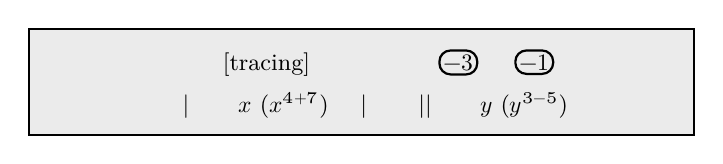
\begin{tikzpicture}[x=1cm, y=1cm, every node/.style={font=\fontsize{8.5pt}{10.5pt}\selectfont, text=black}]
    \draw[black, line width=0.8pt, fill=panelgray] (0,0) rectangle (8.45, 1.35);
    \node[align=center] at (4.225, 0.92) {សម្គាល់ \en{[tracing]}៖ ព័ទ្ធរង្វង់មេគុណ \circbox{-3} និង \circbox{-1}};
    \node[align=center] at (4.225, 0.38) {គូស \en{|} ក្រោម $x$ ($x^{4+7}$) \quad\en{|}\quad គូស \en{||} ក្រោម $y$ ($y^{3-5}$)};
  \end{tikzpicture}
  \end{center}

  \vspace{4pt}
  \begin{tcolorbox}[
    enhanced, sharp corners, colback=panelgray, colframe=black,
    boxrule=0.7pt, boxsep=1pt, top=3.5pt, bottom=3.5pt, left=4.5pt, right=4.5pt
  ]
    \fontsize{7.1pt}{10.0pt}\selectfont
    \textbf{ផ្ទៀងដោយខ្លួនឯង៖}
    \chkbox~ដាក់លេខ \cnum{1}--\cnum{5} \en{|} \chkbox~រក្សា $2=2^1, -x^7=(-1)x^7$ \en{|} \chkbox~រំលង \en{\#7} ក
  \end{tcolorbox}
\end{tcolorbox}%
}

\vspace{3pt}
\noindent
\hwslipFourEXPMUL{ប័ណ្ណទី ១}\hfill\hwslipFourEXPMUL{ប័ណ្ណទី ២}

\vspace{11pt}
\noindent\scissors\ \dotfill\ \textbf{កាត់តាមស្នាមចុចចែកជា ៤ ប័ណ្ណ (\en{Cut Along Dashed Lines})} \dotfill\ \scissors
\vspace{11pt}

\noindent
\hwslipFourEXPMUL{ប័ណ្ណទី ៣}\hfill\hwslipFourEXPMUL{ប័ណ្ណទី ៤}

\end{document}
